% !Mode:: "TeX:UTF-8"
% !TEX encoding = UTF-8 Unicode

%----------------------------------------------------------------------------------------
% 机器翻译:基础与模型
% Machine Translation: Foundations and Models
%
% Copyright 2020
% 肖桐(xiaotong@mail.neu.edu.cn) 朱靖波 (zhujingbo@mail.neu.edu.cn)
%----------------------------------------------------------------------------------------

%----------------------------------------------------------------------------------------
%    CONFIGURATIONS
%----------------------------------------------------------------------------------------

\renewcommand\figurename{图}%将figure改为图
\renewcommand\tablename{表}%将figure改为图
\chapterimage{fig-NEU-6.jpg} % Chapter heading image

%----------------------------------------------------------------------------------------
%	CHAPTER 6
%----------------------------------------------------------------------------------------

\chapter{基于扭曲度和繁衍率的模型}

{\chapterfive}展示了一种基于单词的翻译模型。这种模型的形式非常简单,而且其隐含的词对齐信息具有较好的可解释性。不过,语言翻译的复杂性远远超出人们的想象。语言翻译主要有两方面挑战\ \dash\ 如何对“ 调序”问题进行建模以及如何对“一对多翻译”问题进行建模。一方面,调序是翻译问题中所特有的现象,比如,汉语到日语的翻译中,需要对谓词进行调序。另一方面,一个单词在另一种语言中可能会被翻译为多个连续的词,比如,汉语“ 联合国”翻译到英语会对应三个单词“The United Nations”。这种现象也被称作一对多翻译,它与句子长度预测有着密切的联系。

无论是调序还是一对多翻译,简单的翻译模型(如IBM模型1)都无法对其进行很好的处理。因此,需要考虑对这两个问题单独进行建模。本章将会对机器翻译中两个常用的概念进行介绍\ \dash\ 扭曲度(Distortion)和繁衍率(Fertility)。它们可以被看作是对调序和一对多翻译现象的一种统计描述。基于此,本章会进一步介绍基于扭曲度和繁衍率的翻译模型,建立相对完整的基于单词的统计建模体系。相关的技术和概念在后续章节也会被进一步应用。

%----------------------------------------------------------------------------------------
%    NEW SECTION
%----------------------------------------------------------------------------------------

\sectionnewpage
\section{基于扭曲度的模型}

下面将介绍扭曲度在机器翻译中的定义及使用方法。这也带来了两个新的翻译模型\ \dash\ IBM模型2\upcite{DBLP:journals/coling/BrownPPM94}和HMM\upcite{vogel1996hmm}。

%----------------------------------------------------------------------------------------
%    NEW SUB-SECTION
%----------------------------------------------------------------------------------------
\subsection{什么是扭曲度}

\parinterval {\small\sffamily\bfseries{调序}}(Reordering)是自然语言翻译中特有的语言现象。造成这个现象的主要原因在于不同语言之间语序的差异,比如,汉语是“主谓宾”结构,而日语是“主宾谓”结构。即使在句子整体结构相似的语言上进行翻译,调序也是频繁出现的现象。如图\ref{fig:6-1}所示,当一个主动语态的汉语句子翻译为一个被动语态的英语句子时,如果直接顺序翻译,那么翻译结果“I with you am satisfied”很明显不符合英语语法。这里就需要采取一些方法和手段在翻译过程中对词或短语进行调序,从而得到正确的翻译结果。
%----------------------------------------------
\begin{figure}[htp]
    \centering
%%% outline
%-------------------------------------------------------------------------
\begin{tikzpicture}
\begin{scope}
	\tikzstyle{cand} = [draw,inner sep=4pt,line width=1pt,align=center,drop shadow,minimum height =1.6em,minimum width=4.2em,fill=green!30]
	\tikzstyle{ref} = [draw,inner sep=4pt,line width=1pt,align=center,drop shadow,minimum height =1.6em,minimum width=4.2em,fill=red!30]
		
		\node[align=center,minimum width=2.4em,minimum height=1.6em,minimum width=6em] (n11) at (0,0){源语};
		\node[cand,anchor=west] (n12) at ([xshift=0.0em]n11.east){我};
		\node[cand,anchor=west] (n13) at ([xshift=1em]n12.east){对};
		\node[cand,anchor=west] (n14) at ([xshift=1em]n13.east){你};
		\node[cand,anchor=west] (n15) at ([xshift=1em]n14.east){感到};
		\node[cand,anchor=west] (n16) at ([xshift=1em]n15.east){满意};
		
		\node[align=center,minimum width=2.4em,minimum height=1.6em,anchor=north,minimum width=6em] (n21) at ([yshift=-4em]n11.south){顺序翻译};
		\node[ref,anchor=west] (n22) at ([xshift=0.0em]n21.east){I};
		\node[ref,anchor=west] (n23) at ([xshift=1em]n22.east){with};
		\node[ref,anchor=west] (n24) at ([xshift=1em]n23.east){you};
		\node[ref,anchor=west] (n25) at ([xshift=1em]n24.east){am};
		\node[ref,anchor=west] (n26) at ([xshift=1em]n25.east){satisfied};
		
		\draw[line width=1.2pt,dashed] ([yshift=-0.3em]n12.south) -- ([yshift=0.2em]n22.north);
		\draw[line width=1.2pt,dashed] ([yshift=-0.3em]n13.south) -- ([yshift=0.2em]n23.north);
		\draw[line width=1.2pt,dashed] ([yshift=-0.3em]n14.south) -- ([yshift=0.2em]n24.north);
		\draw[line width=1.2pt,dashed] ([yshift=-0.3em]n15.south) -- ([yshift=0.2em]n25.north);
		\draw[line width=1.2pt,dashed] ([yshift=-0.3em]n16.south) -- ([yshift=0.2em]n26.north);
        \node[anchor=west] at([xshift=5.5em,yshift=-3em]n21.east){\small{(a)顺序翻译对齐结果}};
\end{scope}
\begin{scope}[yshift=-11.5em]
	\tikzstyle{cand} = [draw,inner sep=4pt,line width=1pt,align=center,drop shadow,minimum height =1.6em,minimum width=4.2em,fill=green!30]
	\tikzstyle{ref} = [draw,inner sep=4pt,line width=1pt,align=center,drop shadow,minimum height =1.6em,minimum width=4.2em,fill=red!30]
		
		\node[align=center,minimum width=2.4em,minimum height=1.6em,minimum width=6em] (n11) at (0,0){源语};
		\node[cand,anchor=west] (n12) at ([xshift=0.0em]n11.east){我};
		\node[cand,anchor=west] (n13) at ([xshift=1em]n12.east){对};
		\node[cand,anchor=west] (n14) at ([xshift=1em]n13.east){你};
		\node[cand,anchor=west] (n15) at ([xshift=1em]n14.east){感到};
		\node[cand,anchor=west] (n16) at ([xshift=1em]n15.east){满意};
		
		\node[align=center,minimum width=2.4em,minimum height=1.6em,anchor=north,minimum width=6em] (n21) at ([yshift=-4em]n11.south){调序翻译};
		\node[ref,anchor=west] (n22) at ([xshift=0.0em]n21.east){I};
		\node[ref,anchor=west] (n23) at ([xshift=1em]n22.east){am};
		\node[ref,anchor=west] (n24) at ([xshift=1em]n23.east){satisfied};
		\node[ref,anchor=west] (n25) at ([xshift=1em]n24.east){with};
		\node[ref,anchor=west] (n26) at ([xshift=1em]n25.east){you};
		
		\draw[line width=1.2pt,dashed] ([yshift=-0.3em]n12.south) -- ([yshift=0.2em]n22.north);
		\draw[line width=1.2pt,dashed,out=-40,in=140] ([yshift=-0.3em]n13.south) to ([yshift=0.2em]n25.north);
		\draw[line width=1.2pt,dashed,out=-40,in=140] ([yshift=-0.3em]n14.south) to ([yshift=0.2em]n26.north);
		\draw[line width=1.2pt,dashed,out=-140,in=40] ([yshift=-0.3em]n15.south) to ([yshift=0.2em]n23.north);
		\draw[line width=1.2pt,dashed,out=-140,in=40] ([yshift=-0.3em]n16.south) to ([yshift=0.2em]n24.north);
		\node[anchor=west] at([xshift=5.5em,yshift=-3em]n21.east){\small{(b)调序翻译对齐结果}};
\end{scope}
\end{tikzpicture}
%---------------------------------------------------------------------
    \caption{顺序翻译和调序翻译的实例对比}
    \label{fig:6-1}
\end{figure}
%----------------------------------------------

\parinterval 在对调序问题进行建模的方法中,最基本的是使用调序距离方法。这里,可以假设完全进行顺序翻译时,调序的“代价”是最低的。当调序出现时,可以用调序相对于顺序翻译产生的位置偏移来度量调序的程度,也被称为调序距离。图\ref{fig:6-2}展示了翻译时两种语言中词的对齐矩阵。比如,在图\ref{fig:6-2}(a)中,系统需要跳过“对”和“你”来翻译“感到”和“满意”,之后再回过头翻译“对”和“你”,这样就完成了对单词的调序。这时可以简单地把需要跳过的单词数看作一种距离。

\parinterval 可以看到,调序距离实际上是在度量目标语言词序相对于源语言词序的一种扭曲程度。因此,也常常把这种调序距离称作{\small\sffamily\bfseries{扭曲度}}(Distortion)。调序距离越大对应的扭曲度也越大。比如,可以明显看出图\ref{fig:6-2}(b)中调序的扭曲度要比图\ref{fig:6-2}(a)中调序的扭曲度大,因此\ref{fig:6-2}(b)实例的调序代价也更大。

\parinterval 在机器翻译中使用扭曲度进行翻译建模是一种十分自然的想法。接下来,会介绍两个基于扭曲度的翻译模型,分别是IBM模型2和隐马尔可夫模型。不同于IBM模型1,它们利用了单词的位置信息定义了扭曲度,并将扭曲度融入翻译模型中,使得对翻译问题的建模更加合理。

%----------------------------------------------
\begin{figure}[htp]
    \centering
%%% outline
%-------------------------------------------------------------------------
\newlength{\bc}
\setlength{\bc}{0.5cm}
\begin{tikzpicture}
\begin{scope}
  \filldraw [fill=white,drop shadow] (0,0) rectangle (\bc*5,\bc*5);
    \filldraw [fill=black] (\bc*2,0) rectangle (\bc*3,\bc*1);
    \filldraw [fill=black] (\bc*1,\bc*1) rectangle (\bc*2,\bc*2);
    \filldraw [fill=black] (\bc*4,\bc*2) rectangle (\bc*5,\bc*3);
    \filldraw [fill=black] (\bc*3,\bc*3) rectangle (\bc*4,\bc*4);
    \filldraw [fill=black] (0,\bc*4) rectangle (\bc*1,\bc*5);
    \draw [step=\bc, very thin, color=gray] (0,0) grid (\bc*5,\bc*5);
    \draw [line width=1pt] (0,0) -- (0,\bc*5)--(\bc*5,\bc*5) -- (\bc*5,0) -- (0,0);
    
    \coordinate (o) at (0,\bc*5);
    \node[anchor=east,inner sep=0pt,font=\footnotesize] at([xshift=-0.4em,yshift=-0.25cm]o.west){我};
    \node[anchor=east,inner sep=0pt,font=\footnotesize] at([xshift=-0.4em,yshift=-0.25cm-\bc]o.west){对};
    \node[anchor=east,inner sep=0pt,font=\footnotesize] at([xshift=-0.4em,yshift=-0.25cm-\bc*2]o.west){你};
    \node[anchor=east,inner sep=0pt,font=\footnotesize] at([xshift=-0.4em,yshift=-0.25cm-\bc*3]o.west){感到};
    \node[anchor=east,inner sep=0pt,font=\footnotesize] at([xshift=-0.4em,yshift=-0.25cm-\bc*4]o.west){满意};
     
    \node[anchor=west,inner sep=0pt,font=\footnotesize,rotate=45] at([xshift=0.2cm,yshift=0.4em]o.east){I};
    \node[anchor=west,inner sep=0pt,font=\footnotesize,rotate=45] at([xshift=0.1cm+\bc,yshift=0.4em]o.east){am};
    \node[anchor=west,inner sep=0pt,font=\footnotesize,rotate=45] at([xshift=0.1cm+\bc*2,yshift=0.4em]o.east){satisfied};
    \node[anchor=west,inner sep=0pt,font=\footnotesize,rotate=45] at([xshift=0.1cm+\bc*3,yshift=0.4em]o.east){with};
    \node[anchor=west,inner sep=0pt,font=\footnotesize,rotate=45] at([xshift=0.1cm+\bc*4,yshift=0.4em]o.east){you};
	\node[anchor=east,inner sep=0pt,font=\small] at([xshift=\bc*4.5,yshift=-1.0cm-\bc*4]o.west){(a)对齐实例1};
\end{scope}
\begin{scope}[xshift=17.0em]
    \filldraw [fill=white,drop shadow] (0,0) rectangle (\bc*8,\bc*6);
    \filldraw [fill=black] (0,\bc*5) rectangle (\bc*1,\bc*6);
    \filldraw [fill=black] (\bc*1,\bc*3) rectangle (\bc*2,\bc*4);
    \filldraw [fill=black] (\bc*2,\bc*2) rectangle (\bc*3,\bc*3);
    \filldraw [fill=black] (\bc*3,\bc*2) rectangle (\bc*4,\bc*3);
    \filldraw [fill=black] (\bc*4,\bc*1) rectangle (\bc*5,\bc*2);
    \filldraw [fill=black] (\bc*5,0) rectangle (\bc*6,\bc*1);
    \filldraw [fill=black] (\bc*6,\bc*4) rectangle (\bc*7,\bc*5);
    \filldraw [fill=black] (\bc*7,\bc*4) rectangle (\bc*8,\bc*5);
    \draw [step=\bc, very thin, color=gray] (0,0) grid (\bc*8,\bc*6);
    \draw [line width=1pt] (0,0) -- (0,\bc*6)--(\bc*8,\bc*6) -- (\bc*8,0) -- (0,0);
    
    \coordinate (o) at (0,\bc*6);
    \node[anchor=east,inner sep=0pt,font=\footnotesize] at([xshift=-0.4em,yshift=-0.25cm]o.west){他};
    \node[anchor=east,inner sep=0pt,font=\footnotesize] at([xshift=-0.4em,yshift=-0.25cm-\bc]o.west){每天};
    \node[anchor=east,inner sep=0pt,font=\footnotesize] at([xshift=-0.4em,yshift=-0.25cm-\bc*2]o.west){乘坐};
    \node[anchor=east,inner sep=0pt,font=\footnotesize] at([xshift=-0.4em,yshift=-0.25cm-\bc*3]o.west){地铁};
    \node[anchor=east,inner sep=0pt,font=\footnotesize] at([xshift=-0.4em,yshift=-0.25cm-\bc*4]o.west){去};
    \node[anchor=east,inner sep=0pt,font=\footnotesize] at([xshift=-0.4em,yshift=-0.25cm-\bc*5]o.west){上班};
    
    \node[anchor=west,inner sep=0pt,font=\footnotesize,rotate=45] at([xshift=0.1cm,yshift=0.4em]o.east){He};
    \node[anchor=west,inner sep=0pt,font=\footnotesize,rotate=45] at([xshift=0.1cm+\bc,yshift=0.4em]o.east){takes};
    \node[anchor=west,inner sep=0pt,font=\footnotesize,rotate=45] at([xshift=0.1cm+\bc*2,yshift=0.4em]o.east){the};
    \node[anchor=west,inner sep=0pt,font=\footnotesize,rotate=45] at([xshift=0.1cm+\bc*3,yshift=0.4em]o.east){subway};
    \node[anchor=west,inner sep=0pt,font=\footnotesize,rotate=45] at([xshift=0.1cm+\bc*4,yshift=0.4em]o.east){to};
    \node[anchor=west,inner sep=0pt,font=\footnotesize,rotate=45] at([xshift=0.1cm+\bc*5,yshift=0.4em]o.east){work};
    \node[anchor=west,inner sep=0pt,font=\footnotesize,rotate=45] at([xshift=0.1cm+\bc*6,yshift=0.4em]o.east){every};
    \node[anchor=west,inner sep=0pt,font=\footnotesize,rotate=45] at([xshift=0.1cm+\bc*7,yshift=0.4em]o.east){day};
    \node[anchor=east,inner sep=0pt,font=\small] at([xshift=\bc*6.0,yshift=-1.0cm-\bc*5]o.west){(b)对齐实例2};
\end{scope}
\end{tikzpicture}
%---------------------------------------------------------------------
    \caption{汉语到英语翻译的对齐矩阵}
    \label{fig:6-2}
\end{figure}
%----------------------------------------------

%----------------------------------------------------------------------------------------
%    NEW SUB-SECTION
%----------------------------------------------------------------------------------------
\subsection{IBM模型2}

\parinterval 对于建模来说,IBM模型1很好地化简了翻译问题,但是由于使用了很强的假设,导致模型和实际情况有较大差异。其中一个比较严重的问题是假设词对齐的生成概率服从均匀分布。IBM模型2抛弃了这个假设\upcite{DBLP:journals/coling/BrownPPM94}。它认为词对齐是有倾向性的,它与源语言单词的位置和目标语言单词的位置有关。具体来说,对齐位置$a_j$的生成概率与位置$j$、源语言句子长度$m$和目标语言句子长度$l$有关,形式化表述为:

\begin{eqnarray}
\funp{P}(a_j|a_1^{j-1},s_1^{j-1},m,\seq{t}) & \equiv & a(a_j|j,m,l)
\label{eq:6-1}
\end{eqnarray}

\parinterval 这里还用{\chapterfive}中的例子(图\ref{fig:6-3})来进行说明。在IBM模型1中,“桌子”对齐到目标语言四个位置的概率是一样的。但在IBM模型2中,“桌子”对齐到“table”被形式化为$a(a_j |j,m,l)=a(3|2,3,3)$,意思是对于源语言位置2($j=2$)的词,如果它的源语言和目标语言都是3个词($l=3,m=3$),对齐到目标语言位置3($a_j=3$)的概率是多少?因为$a(a_j|j,m,l)$也是模型需要学习的参数,因此“桌子”对齐到不同目标语言单词的概率也是不一样的。理想的情况下,通过$a(a_j|j,m,l)$,“桌子”对齐到“table”应该得到更高的概率。

%----------------------------------------------
\begin{figure}[htp]
    \centering

%%% outline
%-------------------------------------------------------------------------
\begin{tikzpicture}
{
    \node [anchor=west,inner sep=2pt] (s1) at (0,0) {$s_1$:在};
    \node [anchor=west,inner sep=2pt] (s2) at ([xshift=2em]s1.east) {$s_2$:桌子};
    \node [anchor=west,inner sep=2pt] (s3) at ([xshift=2em]s2.east) {$s_3$:上};

    \node [anchor=north,inner sep=2pt] (t1) at ([yshift=-2.4em]s1.center) {$t_1$:on};
    \node [anchor=north,inner sep=2pt] (t2) at ([yshift=-2.4em]s2.center) {$t_2$:the};
    \node [anchor=north,inner sep=2pt] (t3) at ([yshift=-2.4em]s3.center) {$t_3$:table};
    \node [anchor=east,inner sep=2pt] (t0) at ([xshift=-2.2em]t1.west) {$t_0$};

    \draw [-,dashed,thick] (s1.south) -- (t0.north);
    \draw [-,dashed,thick] (s2.south) -- (t3.north);
    \draw [-,dashed,thick] (s3.south) -- (t1.north);
    }
 \begin{pgfonlayer}{background}
    {
    \path [fill=red!20] (s2.north west) -- (s2.south west) -- (t3.north west) -- (t3.south west) -- (t3.south east) -- (t3.north east) -- (s2.south east) -- (s2.north east) -- (s2.north west);
    }
    \end{pgfonlayer}
    \end{tikzpicture}

%---------------------------------------------------------------------




    \caption{汉译英句对及词对齐}
    \label{fig:6-3}
\end{figure}
%----------------------------------------------

\parinterval IBM模型2的其他假设均与模型1相同,即源语言长度预测概率及源语言单词生成概率被定义为:

\begin{eqnarray}
\funp{P}(m|\seq{t}) & \equiv & \varepsilon \label{eq:s-len-gen-prob} \\
\funp{P}(s_j|a_1^{j},s_1^{j-1},m,\seq{t}) & \equiv & f(s_j|t_{a_j})
\label{eq:s-word-gen-prob}
\end{eqnarray}

把公式\eqref{eq:6-1}、\eqref{eq:s-len-gen-prob}和\eqref{eq:s-word-gen-prob}重新带入公式$\funp{P}(\seq{s},\seq{a}|\seq{t})=\funp{P}(m|\seq{t})\prod_{j=1}^{m}{\funp{P}(a_j|a_1^{j-1},s_1^{j-1},m,\seq{t})}$\\${\funp{P}(s_j|a_1^{j},s_1^{j-1},m,\seq{t})}$ 和$\funp{P}(\seq{s}|\seq{t})= \sum_{\seq{a}}\funp{P}(\seq{s},\seq{a}|\seq{t})$,可以得到IBM模型2的数学描述:
\begin{eqnarray}
\funp{P}(\seq{s}| \seq{t}) & = &  \sum_{\seq{a}}{\funp{P}(\seq{s},\seq{a}| \seq{t})} \nonumber \\
                       & = & \sum_{a_1=0}^{l}{\cdots}\sum _{a_m=0}^{l}{\varepsilon}\prod_{j=1}^{m}{a(a_j|j,m,l)f(s_j|t_{a_j})}
\label{eq:6-4}
\end{eqnarray}

\parinterval 类似于模型1,模型2的表达式\eqref{eq:6-4}也能被拆分为两部分进行理解。第一部分:遍历所有的$\seq{a}$;第二部分:对于每个$\seq{a}$累加对齐概率$\funp{P}(\seq{s},\seq{a}| \seq{t})$,即计算对齐概率$a(a_j|j,m,l)$和词汇翻译概率$f(s_j|t_{a_j})$对于所有源语言位置的乘积。

\parinterval 同样的,模型2的解码及训练优化和模型1的十分相似,在此不再赘述,详细推导过程可以参看{\chapterfive}\ref{IBM-model1}小节解码及计算优化部分。这里直接给出IBM模型2的最终表达式:
\begin{eqnarray}
\funp{P}(\seq{s}| \seq{t}) & = & \varepsilon \prod\limits_{j=1}^{m} \sum\limits_{i=0}^{l} a(i|j,m,l) f(s_j|t_i)
\label{eq:6-5}
\end{eqnarray}


%----------------------------------------------------------------------------------------
%    NEW SUB-SECTION
%----------------------------------------------------------------------------------------

\subsection{隐马尔可夫模型}

\parinterval IBM模型把翻译问题定义为生成词对齐的问题,模型翻译质量的好坏与词对齐有着非常紧密的联系。IBM模型1假设对齐概率仅依赖于目标语言句子长度,即对齐概率服从均匀分布;IBM模型2假设对齐概率与源语言、目标语言的句子长度以及源语言位置和目标语言位置相关。虽然IBM模型2已经覆盖了一部分词对齐问题,但是该模型只考虑到了单词的绝对位置,并未考虑到相邻单词间的关系。图\ref{fig:6-4} 展示了一个简单的实例,可以看到的是,汉语的每个单词都被分配给了英语句子中的每一个单词,但是单词并不是任意分布在各个位置上的,而是倾向于生成簇。也就是说,如果源语言的两个单词位置越近,它们的译文在目标语言句子中的位置也越近。

%----------------------------------------------
\begin{figure}[htp]
    \centering

%%% outline
%-------------------------------------------------------------------------


\begin{tikzpicture}

\begin{scope}
\node [anchor=west] (s1) at (0,0) {\small{$s_1$}:我};
\node [anchor=west] (s2) at ([xshift=0.5em]s1.east) {\small{$s_2$}:对};
\node [anchor=west] (s3) at ([xshift=0.5em]s2.east) {\small{$s_3$}:你};
\node [anchor=west] (s4) at ([xshift=0.5em]s3.east) {\small{$s_4$}:感到};
\node [anchor=west] (s5) at ([xshift=0.5em]s4.east) {\small{$s_5$}:满意};
\end{scope}

\begin{scope}[yshift=-3.5em]
\node [anchor=west] (t1) at (0.45em,0) {\small{$t_1$}:I};
\node [anchor=west] (t2) at ([xshift=1.0em,yshift=0.0em]t1.east) {\small{$t_2$}:am};
\node [anchor=west] (t3) at ([xshift=0.3em,yshift=0.0em]t2.east) {\small{$t_3$}:satisfied};
\node [anchor=west] (t4) at ([xshift=0.3em]t3.east) {\small{$t_4$}:with};
\node [anchor=west] (t5) at ([xshift=0.3em,yshift=-0.0em]t4.east) {\small{$t_5$}:you};
\end{scope}


\draw [-,thick,dashed] (s1.south) -- (t1.north);
\draw [-,thick,dashed] (s4.south) -- ([yshift=0.3em]t2.north);
\draw [-,thick,dashed] (s2.south) ..controls +(south:1em) and +(north:1em).. (t4.north);
\draw [-,thick,dashed] (s3.south) ..controls +(south:0.5em) and +(north:1.5em).. (t5.north);
\draw [-,thick,dashed] (s5.south) -- (t3.north);

\end{tikzpicture}


%---------------------------------------------------------------------




    \caption{汉译英句对及对齐}
    \label{fig:6-4}
\end{figure}
%----------------------------------------------

\parinterval 针对此问题,基于HMM的词对齐模型抛弃了IBM模型1-2的绝对位置假设,将一阶隐马尔可夫模型用于词对齐问题\upcite{vogel1996hmm}。HMM词对齐模型认为,单词与单词之间并不是毫无联系的,对齐概率应该取决于对齐位置的差异而不是本身单词所在的位置。具体来说,位置$j$的对齐概率$a_j$与前一个位置$j-1$的对齐位置$a_{j-1}$和译文长度$l$有关,形式化的表述为:
\begin{eqnarray}
\funp{P}(a_{j}|a_{1}^{j-1},s_{1}^{j-1},m,\seq{t})& \equiv & \funp{P}(a_{j}|a_{j-1},l)
\label{eq:6-6}
\end{eqnarray}

\parinterval 这里用图\ref{fig:6-4}的例子对公式进行说明。在IBM模型1-2中,单词的对齐都是与单词所在的绝对位置有关。但在HMM词对齐模型中,“你”对齐到“you”被形式化为$\funp{P}(a_{j}|a_{j-1},l)= P(5|4,5)$,意思是对于源语言位置$3(j=3)$上的单词,如果它的译文是第5个目标语言单词,上一个对齐位置是$4(a_{2}=4)$,对齐到目标语言位置$5(a_{j}=5)$的概率是多少?理想的情况下,通过$\funp{P}(a_{j}|a_{j-1},l)$,“你”对齐到“you”应该得到更高的概率,并且由于源语言单词“对”和“你”距离很近,因此其对应的对齐位置“with”和“you”的距离也应该很近。

\parinterval 把公式$\funp{P}(s_j|a_1^{j},s_1^{j-1},m,\seq{t}) \equiv f(s_j|t_{a_j})$和\eqref{eq:6-6}重新带入公式$\funp{P}(\seq{s},\seq{a}|\seq{t})=\funp{P}(m|\seq{t})$\\$\prod_{j=1}^{m}{\funp{P}(a_j|a_1^{j-1},s_1^{j-1},m,\seq{t})\funp{P}(s_j|a_1^{j},s_1^{j-1},m,\seq{t})}$和$\funp{P}(\seq{s}|\seq{t})= \sum_{\seq{a}}\funp{P}(\seq{s},\seq{a}|\seq{t})$,可得HMM词对齐模型的数学描述:
\begin{eqnarray}
\funp{P}(\seq{s}| \seq{t})& =& \sum_{\seq{a}}{\funp{P}(m|\seq{t})}\prod_{j=1}^{m}{\funp{P}(a_{j}|a_{j-1},l)f(s_{j}|t_{a_j})}
\label{eq:6-7}
\end{eqnarray}

\parinterval 此外,为了使得HMM的对齐概率$\funp{P}(a_{j}|a_{j-1},l)$满足归一化的条件,这里还假设其对齐概率只取决于$a_{j}-a_{j-1}$,即:
\begin{eqnarray}
\funp{P}(a_{j}|a_{j-1},l)& = & \frac{\mu(a_{j}-a_{j-1})}{\sum_{i=1}^{l}{\mu(i-a_{j-1})}}
\label{eq:6-8}
\end{eqnarray}

\noindent 其中,$\mu( \cdot )$是隐马尔可夫模型的参数,可以通过训练得到。

\parinterval 需要注意的是,公式\eqref{eq:6-7}之所以被看作是一种隐马尔可夫模型,是由于其形式与标准的一阶隐马尔可夫模型无异。$\funp{P}(a_{j}|a_{j-1},l)$可以被看作是一种状态转移概率,$f(s_{j}|t_{a_j})$可以被看作是一种发射概率。关于隐马尔可夫模型具体的数学描述也可参考{\chapterthree}中的相关内容。

%----------------------------------------------------------------------------------------
%    NEW SECTION
%----------------------------------------------------------------------------------------

\sectionnewpage
\section{基于繁衍率的模型}

下面介绍翻译中的一对多问题,以及这个问题所带来的句子长度预测问题。

%----------------------------------------------------------------------------------------
%    NEW SUB-SECTION
%----------------------------------------------------------------------------------------

\subsection{什么是繁衍率}

\parinterval 从前面的介绍可知,IBM模型1和模型2把不同的源语言单词看作相互独立的单元来进行词对齐和翻译。换句话说,即使某个源语言短语中的两个单词都对齐到同一个目标语单词,它们之间也是相互独立的。这样IBM模型1和模型2对于多个源语言单词对齐到同一个目标语单词的情况并不能很好地进行描述。

\parinterval 这里将会给出另一个翻译模型,能在一定程度上解决上面提到的问题\upcite{DBLP:journals/coling/BrownPPM94,och2003systematic}。该模型把目标语言生成源语言的过程分解为如下几个步骤:首先,确定每个目标语言单词生成源语言单词的个数,这里把它称为{\small\sffamily\bfseries{繁衍率}}\index{繁衍率}或{\small\sffamily\bfseries{产出率}}\index{产出率}(Fertility)\index{Fertility};其次,决定目标语言句子中每个单词生成的源语言单词都是什么,即决定生成的第一个源语言单词是什么,生成的第二个源语言单词是什么,以此类推。这样每个目标语言单词就对应了一个源语言单词列表;最后把各组源语言单词列表中的每个单词都放置到合适的位置上,完成目标语言译文到源语言句子的生成。

%----------------------------------------------
\begin{figure}[htp]
    \centering
%%% outline
%-------------------------------------------------------------------------
\begin{tikzpicture}

{
{
\node [anchor=north west] (st) at (0,0) {$\seq{s}$};
\node [anchor=north] (taut) at ([yshift=-3em]st.south) {\sffamily\bfseries{$\tau$}};
\node [anchor=north] (phit) at ([yshift=-3em]taut.south) {\sffamily\bfseries{$\phi$}};
\node [anchor=north] (tt) at ([yshift=-3em]phit.south) {$\seq{t}$};
}
{\scriptsize
\node [anchor=west,minimum height=2.5em,minimum width=5.0em] (sf1) at ([xshift=1em]st.east) {};
\node [rectangle,draw,anchor=west,line width=1pt,minimum height=2.5em,minimum width=5.0em,fill=green!30,drop shadow] (s1) at ([xshift=2.5em]sf1.east) {科学家};
\node [rectangle,draw,anchor=west,line width=1pt,minimum height=2.5em,minimum width=5.0em,fill=green!30,drop shadow] (s2) at ([xshift=2.5em]s1.east) {们};
\node [rectangle,draw,anchor=west,line width=1pt,minimum height=2.5em,minimum width=5.0em,fill=green!30,drop shadow] (s3) at ([xshift=2.5em]s2.east) {并不};
\node [rectangle,draw,anchor=west,line width=1pt,minimum height=2.5em,minimum width=5.0em,fill=green!30,drop shadow] (s4) at ([xshift=2.5em]s3.east) {知道};
}


{\scriptsize
\node [anchor=west] (tau11) at ([xshift=1.24em]taut.east) {$\tau_0$\; \tiny{1.NULL}};
\begin{pgfonlayer}{background}
\node [rounded rectangle,draw,line width=1pt,minimum height=3.0em,minimum width=7.0em,fill=red!30,drop shadow] (tau1) [fit = (tau11)] {};
\end{pgfonlayer}

\node [anchor=west] (tau21) at ([xshift=1.575em]tau1.east) {$\tau_1$\;};
\node [anchor=west] (tau22) at ([yshift=-0.2em,xshift=-0.5em]tau21.north east) {\tiny{1.科学家}};
\node [anchor=west] (tau23) at ([yshift=0.2em,xshift=-0.5em]tau21.south east) {\tiny{2.们}};
\begin{pgfonlayer}{background}
\node [rounded rectangle,draw,line width=1pt,minimum height=3.0em,minimum width=7.0em,fill=red!30,drop shadow] (tau2)[fit = (tau21) (tau22) (tau23)] {};
\end{pgfonlayer}

\node [anchor=west] (tau31) at ([xshift=1.997em]tau2.east) {$\tau_2$\; \tiny{1.NULL}};
\begin{pgfonlayer}{background}
\node [rounded rectangle,draw,line width=1pt,minimum height=3.0em,minimum width=7.0em,fill=red!30,drop shadow] (tau3) [fit = (tau31)] {};
\end{pgfonlayer}

\node [anchor=west] (tau41) at ([xshift=2.153em]tau3.east) {$\tau_3$\; \tiny{1.并不}};
\begin{pgfonlayer}{background}
\node [rounded rectangle,draw,line width=1pt,minimum height=3.0em,minimum width=7.0em,fill=red!30,drop shadow] (tau4) [fit = (tau41)] {};
\end{pgfonlayer}

\node [anchor=west] (tau51) at ([xshift=2.1525em]tau4.east) {$\tau_4$\; \tiny{1.知道}};
\begin{pgfonlayer}{background}
\node [rounded rectangle,draw,line width=1pt,minimum height=3.0em,minimum width=7.0em,fill=red!30,drop shadow] (tau5) [fit = (tau51)] {};
\end{pgfonlayer}
}


{\scriptsize
\node [anchor=west] (phi11) at ([xshift=2.3em]phit.east) {$\phi_0$\ 0};
\begin{pgfonlayer}{background}
\node [rounded rectangle,draw,line width=1pt,minimum height=3.0em,minimum width=7.0em,fill=blue!30,drop shadow] (phi1) [fit = (phi11)] {};
\end{pgfonlayer}

\node [anchor=west] (phi21) at ([xshift=2.867em]phi1.east) {$\phi_1$\ 2};
\begin{pgfonlayer}{background}
\node [rounded rectangle,draw,line width=1pt,minimum height=3.0em,minimum width=7.0em,fill=blue!30,drop shadow] (phi2) [fit = (phi21)] {};
\end{pgfonlayer}

\node [anchor=west] (phi31) at ([xshift=3.087em]phi2.east) {$\phi_2$\ 0};
\begin{pgfonlayer}{background}
\node [rounded rectangle,draw,line width=1pt,minimum height=3.0em,minimum width=7.0em,fill=blue!30,drop shadow] (phi3) [fit = (phi31)] {};
\end{pgfonlayer}

\node [anchor=west] (phi41) at ([xshift=3.086em]phi3.east) {$\phi_3$\ 1};
\begin{pgfonlayer}{background}
\node [rounded rectangle,draw,line width=1pt,minimum height=3.0em,minimum width=7.0em,fill=blue!30,drop shadow] (phi4) [fit = (phi41)] {};
\end{pgfonlayer}

\node [anchor=west] (phi51) at ([xshift=3.086em]phi4.east) {$\phi_4$\ 1};
\begin{pgfonlayer}{background}
\node [rounded rectangle,draw,line width=1pt,minimum height=3.0em,minimum width=7.0em,fill=blue!30,drop shadow] (phi5) [fit = (phi51)] {};
\end{pgfonlayer}

}

\draw [->,thick,dashed] ([yshift=-1.4em]st.south west) -- ([xshift=0.8em,yshift=-1em]s4.south east);
\draw [->,thick,dashed] ([yshift=-5.8em]st.south west) -- ([xshift=0.8em,yshift=-5.4em]s4.south east);
\draw [->,thick,dashed] ([yshift=-10.3em]st.south west) -- ([xshift=0.8em,yshift=-9.9em]s4.south east);

{\scriptsize
\node [rectangle,draw,anchor=north,line width=1pt,minimum height=2.5em,minimum width=5.0em,fill=yellow!30,drop shadow] (t1) at ([xshift=0.182em,yshift=-15em]sf1.south) {$t_0$};
\node [rectangle,draw,anchor=north,line width=1pt,minimum height=2.5em,minimum width=5.0em,fill=yellow!30,drop shadow] (t2) at ([yshift=-15em]s1.south) {Scientists};
\node [rectangle,draw,anchor=north,line width=1pt,minimum height=2.5em,minimum width=5.0em,fill=yellow!30,drop shadow] (t3) at ([yshift=-15em]s2.south) {do};
\node [rectangle,draw,anchor=north,line width=1pt,minimum height=2.5em,minimum width=5.0em,fill=yellow!30,drop shadow] (t4) at ([yshift=-15em]s3.south) {not};
\node [rectangle,draw,anchor=north,line width=1pt,minimum height=2.5em,minimum width=5.0em,fill=yellow!30,drop shadow] (t5) at ([yshift=-15em]s4.south) {know};
}
%第一层连线
\draw [->,thick] (tau2.north) -- (s1.south);
\draw [->,thick] (tau4.north) -- (s3.south);
\draw [->,thick] (tau5.north) -- (s4.south);
\draw [->,thick] (tau23.east) -- (s2.south);
%第二层连线
\draw [->,thick] (phi1.north) -- (tau1.south);
\draw [->,thick] (phi2.north) -- (tau2.south);
\draw [->,thick] (phi3.north) -- (tau3.south);
\draw [->,thick] (phi4.north) -- (tau4.south);
\draw [->,thick] (phi5.north) -- (tau5.south);
%第三层连线
\draw [->,thick] (t1.north) -- (phi1.south);
\draw [->,thick] (t2.north) -- (phi2.south);
\draw [->,thick] (t3.north) -- (phi3.south);
\draw [->,thick] (t4.north) -- (phi4.south);
\draw [->,thick] (t5.north) -- (phi5.south);

{\scriptsize
\node [anchor=west] (sent11) at ([xshift=1em,yshift=-0.3em]s4.south east) {把这些元语};
\node [anchor=west] (sent12) at ([yshift=-1em]sent11.west) {言单词放在};
\node [anchor=west] (sent13) at ([yshift=-1em]sent12.west) {合适的位置};
\node [anchor=west] (sent21) at ([yshift=-4.6em]sent13.west) {确定生成元};
\node [anchor=west] (sent22) at ([yshift=-1em]sent21.west) {语言单词};
\node [anchor=west] (sent31) at ([yshift=-4.6em]sent22.west) {确定生成元};
\node [anchor=west] (sent32) at ([yshift=-1em]sent31.west) {语言单词的};
\node [anchor=west] (sent33) at ([yshift=-1em]sent32.west) {个数};
}

{\scriptsize
\node [anchor=west] (f1) at ([yshift=-2em]t1.south west) {$\phi_{0}=0,\phi_{1}=2,\phi_{3}=0,\phi_{4}=1$};
\node [anchor=west] (f2) at ([yshift=-2em]f1.west) {$\tau_{0}=\{ \},\tau_{1}=\{ \tau_{11}=' \textrm{科学家}',\tau_{12}=' \textrm{们}' \},\phi_{3}=\{ \tau_{31}=' \textrm{并不}' \},\phi_{4}=\{ \tau_{41}=' \textrm{知道}' \}$};
\node [anchor=west] (f3) at ([yshift=-2em]f2.west) {$\pi_{0}=\{ \},\pi_{1}=\{\pi_{11}=1,\pi_{12}=2\},\pi_{2}=\{ \},\pi_{3}=\{\pi_{31}=3\},\pi_{4}=\{\pi_{41}=4\}$};
}

}
\end{tikzpicture}
%---------------------------------------------------------------------

   \caption{基于产出率的翻译模型执行过程}
   \label{fig:6-5}
\end{figure}
%----------------------------------------------

\parinterval 对于句对$(\seq{s},\seq{t})$,令$\varphi$表示产出率,同时令${\tau}$表示每个目标语言单词对应的源语言单词列表。图{\ref{fig:6-5}}描述了一个英语句子生成汉语句子的过程。

\begin{itemize}
\vspace{0.3em}
\item 首先,对于每个英语单词$t_i$确定它的产出率$\varphi_{i}$。比如“Scientists”的产出率是2,可表示为${\varphi}_{1}=2$。这表明它会生成2个汉语单词;
\vspace{0.3em}
\item 其次,确定英语句子中每个单词生成的汉语单词列表。比如“Scientists”生成“科学家”和“们”两个汉语单词,可表示为${\tau}_1=\{{\tau}_{11}=\textrm{“科学家”},{\tau}_{12}=\textrm{“们”}\}$。 这里用特殊的空标记NULL表示翻译对空的情况;
\vspace{0.3em}
\item 最后,把生成的所有汉语单词放在合适的位置。比如“科学家”和“们”分别放在$\seq{s}$的位置1和位置2。可以用符号$\pi$记录生成的单词在源语言句子$\seq{s}$中的位置。比如“Scientists” 生成的汉语单词在$\seq{s}$ 中的位置表示为${\pi}_{1}=\{{\pi}_{11}=1,{\pi}_{12}=2\}$。
\end{itemize}

\parinterval 为了表述清晰,这里重新说明每个符号的含义。$\seq{s}$、$\seq{t}$、$m$和$l$分别表示源语言句子、目标语言译文、源语言单词数量以及译文单词数量。$\mathbf{\varphi}$、$\mathbf{\tau}$ 和$\mathbf{\pi}$分别表示产出率、生成的源语言单词以及它们在源语言句子中的位置。${\varphi}_{i}$表示第$i$个目标语言单词$t_i$的产出率。${\tau}_{i}$和${\pi}_i$ 分别表示$t_i$生成的源语言单词列表及其在源语言句子$\seq{s}$中的位置列表。

\parinterval 可以看出,一组$\tau$和$\pi$(记为$<\tau,\pi>$)可以决定一个对齐$\seq{a}$和一个源语句子$\seq{s}$。

\noindent 相反的,一个对齐$\seq{a}$和一个源语句子$\seq{s}$可以对应多组$<\tau,\pi>$。如图\ref{fig:6-6}所示,不同的$<\tau,\pi>$对应同一个源语言句子和词对齐。它们的区别在于目标语单词“Scientists”生成的源语言单词“科学家”和“ 们”的顺序不同。这里把不同的$<\tau,\pi>$对应到的相同的源语句子$\seq{s}$和对齐$\seq{a}$记为$<\seq{s},\seq{a}>$。因此计算$\funp{P}(\seq{s},\seq{a}| \seq{t})$时需要把每个可能结果的概率加起来,如下:
\begin{eqnarray}
\funp{P}(\seq{s},\seq{a}| \seq{t}) & = & \sum_{{<\tau,\pi>}\in{<\seq{s},\seq{a}>}}{\funp{P}(\tau,\pi|\seq{t}) }
\label{eq:6-9}
\end{eqnarray}

%----------------------------------------------
\begin{figure}[htp]
    \centering
%%% outline
%-------------------------------------------------------------------------
\begin{tikzpicture}
\begin{scope}
{
\node [anchor=north west] (st) at (0,0) {\color{white}$\mathbf{s}$};
\node [anchor=north] (taut) at ([yshift=-3em]st.south) {\color{white}\sffamily\bfseries{$\tau$}};
\node [anchor=north] (phit) at ([yshift=-3em]taut.south) {\color{white}\sffamily\bfseries{$\phi$}};
\node [anchor=north] (tt) at ([yshift=-3em]phit.south) {\color{white}$\mathbf{t}$};
}
{\scriptsize
\node [anchor=west,minimum height=2.5em,minimum width=5.0em] (sf1) at ([xshift=1em]st.east) {};
\node [rectangle,draw,anchor=west,line width=1pt,minimum height=2.5em,minimum width=5.0em,fill=green!30,drop shadow] (s1) at ([xshift=2.5em]sf1.east) {科学家};
\node [rectangle,draw,anchor=west,line width=1pt,minimum height=2.5em,minimum width=5.0em,fill=green!30,drop shadow] (s2) at ([xshift=2.5em]s1.east) {们};
\node [rectangle,draw,anchor=west,line width=1pt,minimum height=2.5em,minimum width=5.0em,fill=green!30,drop shadow] (s3) at ([xshift=2.5em]s2.east) {并不};
\node [rectangle,draw,anchor=west,line width=1pt,minimum height=2.5em,minimum width=5.0em,fill=green!30,drop shadow] (s4) at ([xshift=2.5em]s3.east) {知道};
}


{\scriptsize
\node [anchor=west] (tau11) at ([xshift=1.24em]taut.east) {$\tau_0$\; \tiny{1.NULL}};
\begin{pgfonlayer}{background}
\node [rounded rectangle,draw,line width=1pt,minimum height=3.0em,minimum width=7.0em,fill=red!30,drop shadow] (tau1) [fit = (tau11)] {};
\end{pgfonlayer}

\node [anchor=west] (tau21) at ([xshift=1.575em]tau1.east) {$\tau_1$\;};
\node [anchor=west] (tau22) at ([yshift=-0.2em,xshift=-0.5em]tau21.north east) {\tiny{1.科学家}};
\node [anchor=west] (tau23) at ([yshift=0.2em,xshift=-0.5em]tau21.south east) {\tiny{2.们}};
\begin{pgfonlayer}{background}
\node [rounded rectangle,draw,line width=1pt,minimum height=3.0em,minimum width=7.0em,fill=red!30,drop shadow] (tau2)[fit = (tau21) (tau22) (tau23)] {};
\end{pgfonlayer}

\node [anchor=west] (tau31) at ([xshift=1.997em]tau2.east) {$\tau_2$\; \tiny{1.NULL}};
\begin{pgfonlayer}{background}
\node [rounded rectangle,draw,line width=1pt,minimum height=3.0em,minimum width=7.0em,fill=red!30,drop shadow] (tau3) [fit = (tau31)] {};
\end{pgfonlayer}

\node [anchor=west] (tau41) at ([xshift=2.153em]tau3.east) {$\tau_3$\; \tiny{1.并不}};
\begin{pgfonlayer}{background}
\node [rounded rectangle,draw,line width=1pt,minimum height=3.0em,minimum width=7.0em,fill=red!30,drop shadow] (tau4) [fit = (tau41)] {};
\end{pgfonlayer}

\node [anchor=west] (tau51) at ([xshift=2.1525em]tau4.east) {$\tau_4$\; \tiny{1.知道}};
\begin{pgfonlayer}{background}
\node [rounded rectangle,draw,line width=1pt,minimum height=3.0em,minimum width=7.0em,fill=red!30,drop shadow] (tau5) [fit = (tau51)] {};
\end{pgfonlayer}
}

{
\node [anchor=north] (d1) at ([yshift=-6.02em]sf1.south) {$...$};
\node [anchor=north] (d2) at ([yshift=-6em]s1.south) {$...$};
\node [anchor=north] (d31) at ([yshift=-6em]s2.south) {$...$};
\node [anchor=north] (d32) at ([xshift=0.2em]d31.south) {\footnotesize{${<{\tau,\pi}>}_1$}};
\node [anchor=north] (d4) at ([yshift=-6em]s3.south) {$...$};
\node [anchor=north] (d5) at ([yshift=-6em]s4.south) {$...$};
}

\draw [->,thick,dashed] ([yshift=1em]tau1.north west) -- ([yshift=1em]tau5.north east);
\draw [->,thick,dashed] ([yshift=-1em]tau1.south west) -- ([yshift=-1em]tau5.south east);
%第一层连线
\draw [->,thick] (tau2.north) -- (s1.south);
\draw [->,thick] (tau4.north) -- (s3.south);
\draw [->,thick] (tau5.north) -- (s4.south);
\draw [->,thick] (tau23.east) -- (s2.south);
%第二层连线
\draw [->,thick] (d1.north) -- ([yshift=-4.48em]sf1.south);
\draw [->,thick] (d2.north) -- ([yshift=-4.45em]s1.south);
\draw [->,thick] (d31.north) -- ([yshift=-4.45em]s2.south);
\draw [->,thick] (d4.north) -- ([yshift=-4.45em]s3.south);
\draw [->,thick] (d5.north) -- ([yshift=-4.45em]s4.south);

\end{scope}

{\scriptsize
\node [anchor=west,minimum height=2.5em,minimum width=5.0em] (sf12) at ([yshift=-15.0em,xshift=1em]st.east) {};
\node [rectangle,draw,anchor=west,line width=1pt,minimum height=2.5em,minimum width=5.0em,fill=green!30,drop shadow] (s12) at ([xshift=2.5em]sf12.east) {科学家};
\node [rectangle,draw,anchor=west,line width=1pt,minimum height=2.5em,minimum width=5.0em,fill=green!30,drop shadow] (s22) at ([xshift=2.5em]s12.east) {们};
\node [rectangle,draw,anchor=west,line width=1pt,minimum height=2.5em,minimum width=5.0em,fill=green!30,drop shadow] (s32) at ([xshift=2.5em]s22.east) {并不};
\node [rectangle,draw,anchor=west,line width=1pt,minimum height=2.5em,minimum width=5.0em,fill=green!30,drop shadow] (s42) at ([xshift=2.5em]s32.east) {知道};
}


{\scriptsize
\node [anchor=west] (tau112) at ([yshift=-15.0em,xshift=1.24em]taut.east) {$\tau_0$\; \tiny{1.NULL}};
\begin{pgfonlayer}{background}
\node [rounded rectangle,draw,line width=1pt,minimum height=3.0em,minimum width=6.8em,fill=red!30,drop shadow] (tau12) [fit = (tau112)] {};
\end{pgfonlayer}

\node [anchor=west] (tau212) at ([xshift=1.6762em]tau12.east) {$\tau_1$\;};
\node [anchor=west] (tau222) at ([yshift=-0.2em,xshift=-0.5em]tau212.north east) {\tiny{1.们}};
\node [anchor=west] (tau232) at ([yshift=0.2em,xshift=-0.5em]tau212.south east) {\tiny{2.科学家}};
\begin{pgfonlayer}{background}
\node [rounded rectangle,draw,line width=1pt,minimum height=3.0em,minimum width=6.8em,fill=yellow!30,drop shadow] (tau22)[fit = (tau212) (tau222) (tau232)] {};
\end{pgfonlayer}

\node [anchor=west] (tau312) at ([xshift=1.997em]tau22.east) {$\tau_2$\; \tiny{1.NULL}};
\begin{pgfonlayer}{background}
\node [rounded rectangle,draw,line width=1pt,minimum height=3.0em,minimum width=6.8em,fill=red!30,drop shadow] (tau32) [fit = (tau312)] {};
\end{pgfonlayer}

\node [anchor=west] (tau412) at ([xshift=1.9555em]tau32.east) {$\tau_3$\; \tiny{1.并不}};
\begin{pgfonlayer}{background}
\node [rounded rectangle,draw,line width=1pt,minimum height=3.0em,minimum width=6.8em,fill=red!30,drop shadow] (tau42) [fit = (tau412)] {};
\end{pgfonlayer}

\node [anchor=west] (tau512) at ([xshift=2.2525em]tau42.east) {$\tau_4$\; \tiny{1.知道}};
\begin{pgfonlayer}{background}
\node [rounded rectangle,draw,line width=1pt,minimum height=3.0em,minimum width=6.8em,fill=red!30,drop shadow] (tau52) [fit = (tau512)] {};
\end{pgfonlayer}
}
{
\node [anchor=north] (d12) at ([yshift=-6.02em]sf12.south) {$...$};
\node [anchor=north] (d22) at ([yshift=-6em]s12.south) {$...$};
\node [anchor=north] (d312) at ([yshift=-6em]s22.south) {$...$};
\node [anchor=north] (d322) at ([xshift=0.2em]d312.south) {\footnotesize{${<{\tau,\pi}>}_2$}};
\node [anchor=north] (d42) at ([yshift=-6em]s32.south) {$...$};
\node [anchor=north] (d52) at ([yshift=-6em]s42.south) {$...$};
}

\draw [->,thick,dashed] ([yshift=1em]tau12.north west) -- ([yshift=1em]tau52.north east);
\draw [->,thick,dashed] ([yshift=-1em]tau12.south west) -- ([yshift=-1em]tau52.south east);
%第一层连线
\draw [->,thick] (tau22.north) -- (s12.south);
\draw [->,thick] (tau42.north) -- (s32.south);
\draw [->,thick] (tau52.north) -- (s42.south);
\draw [->,thick] (tau232.east) -- (s22.south);
%第二层连线
\draw [->,thick] (d12.north) -- ([yshift=-4.48em]sf12.south);
\draw [->,thick] (d22.north) -- ([yshift=-4.45em]s12.south);
\draw [->,thick] (d312.north) -- ([yshift=-4.45em]s22.south);
\draw [->,thick] (d42.north) -- ([yshift=-4.45em]s32.south);
\draw [->,thick] (d52.north) -- ([yshift=-4.45em]s42.south);


%\end{scope}

\end{tikzpicture}
%---------------------------------------------------------------------

   \caption{不同$\tau$和$\pi$对应相同的源语言句子和词对齐的情况}
   \label{fig:6-6}
\end{figure}
%----------------------------------------------


\parinterval 不过$<\seq{s},\seq{a}>$中有多少组$<\tau,\pi>$呢?通过图\ref{fig:6-5}中的例子,可以推出$<\seq{s},\seq{a}>$应该包含$\prod_{i=0}^{l}{\varphi_i !}$个不同的二元组$<\tau,\pi>$。 这是因为在给定源语言句子和词对齐时,对于每一个$\tau_i$都有$\varphi_{i}!$种排列。


\parinterval 进一步,$\funp{P}(\tau,\pi|\seq{t})$可以被表示如图\ref{fig:6-7}的形式。其中$\tau_{i1}^{k-1}$表示$\tau_{i1}\cdots \tau_{i(k-1)}$,$\pi_{i1}^{ k-1}$表示$\pi_{i1}\cdots \pi_{i(k-1)}$。可以把图\ref{fig:6-7}中的公式分为5个部分,并用不同的序号和颜色进行标注。每部分的具体含义是:

%----------------------------------------------
\begin{figure}[htp]
    \centering



%%% outline
%-------------------------------------------------------------------------


%%% 简易机器翻译系统 - step 3 decoding - example


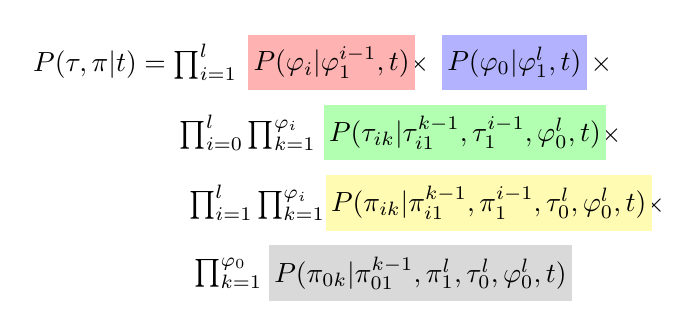
\begin{tikzpicture}



\node [anchor=west,inner sep=2pt,minimum height=2.5em] (eq1) at (0,0) {${\funp{P}(\tau,\pi|\seq{t}) =  \prod_{i=1}^{l}\hspace{6.0em} \times \ \hspace{5.5em}\times}$};
\node [anchor=north west,inner sep=2pt,minimum height=2.5em] (eq2) at ([xshift=-16.06em,yshift=0.0em]eq1.south east) {${\prod_{i=0}^l{\prod_{k=1}^{\varphi_i}\hspace{9.6em}} \ \ \times}$};
\node [anchor=north west,inner sep=2pt,minimum height=2.5em] (eq3) at ([xshift=-16.05em,yshift=0.0em]eq2.south east) {${\prod_{i=1}^l{\prod_{k=1}^{\varphi_i}}\hspace{11.5em} \times}$};
\node [anchor=north west,inner sep=2pt,minimum height=2.5em] (eq4) at ([xshift=-17.44em,yshift=0.0em]eq3.south east) {{${\prod_{k=1}^{\varphi_0}}$}};

\node [anchor=west,inner sep=2pt,minimum height=2.0em,fill=red!30] (part1) at ([xshift=-13.4em,yshift=0.0em]eq1.east) {{${\funp{P}(\varphi_i|\varphi_{1}^{i-1},\seq{t})}$}};
\node [anchor=west,inner sep=2pt,minimum height=2.0em,fill=blue!30] (part2) at ([xshift=-6.4em,yshift=0.0em]eq1.east) {{${\funp{P}(\varphi_0|\varphi_{1}^{l},\seq{t})}$}};
\node [anchor=west,inner sep=2pt,minimum height=2.0em,fill=green!30] (part3) at ([xshift=-11em,yshift=0.0em]eq2.east) {{${\funp{P}(\tau_{ik}|\tau_{i1}^{k-1},\tau_{1}^{i-1},\varphi_{0}^{l},\seq{t} )}$}};
\node [anchor=west,inner sep=2pt,minimum height=2.0em,fill=yellow!30] (part4) at ([xshift=-12.5em,yshift=0.0em]eq3.east) {{${\funp{P}(\pi_{ik}|\pi_{i1}^{k-1},\pi_{1}^{i-1},\tau_{0}^{l},\varphi_{0}^{l},\seq{t} )}$}};
\node [anchor=west,inner sep=2pt,minimum height=2.0em,fill=gray!30] (part5) at ([xshift=0.0em,yshift=0.0em]eq4.east) {{${\funp{P}(\pi_{0k}|\pi_{01}^{k-1},\pi_{1}^{l},\tau_{0}^{l},\varphi_{0}^{l},\seq{t} )}$}};


\end{tikzpicture}




































   \caption{{$\funp{P}(\tau,\pi|t)$}的详细表达式}
\setlength{\belowcaptionskip}{-0.5em}
   \label{fig:6-7}
\end{figure}
%----------------------------------------------

\begin{itemize}
\item 第一部分:对每个$i\in[1,l]$的目标语单词的产出率建模({\color{red!70} 红色}),即$\varphi_i$的生成概率。它依赖于$\seq{t}$和区间$[1,i-1]$的目标语单词的产出率$\varphi_1^{i-1}$。\footnote{这里约定,当$i=1$ 时,$\varphi_1^0$ 表示空。}
\vspace{0.5em}
\item 第二部分:对$i=0$时的产出率建模({\color{blue!70} 蓝色}),即空标记$t_0$的产出率生成概率。它依赖于$\seq{t}$和区间$[1,i-1]$的目标语单词的产出率$\varphi_1^l$。
\vspace{0.5em}
\item 第三部分:对词汇翻译建模({\color{green!70} 绿色}),目标语言单词$t_i$生成第$k$个源语言单词$\tau_{ik}$时的概率,依赖于$\seq{t}$、所有目标语言单词的产出率$\varphi_0^l$、区间$i\in[1,l]$的目标语言单词生成的源语言单词$\tau_1^{i-1}$和目标语单词$t_i$生成的前$k$个源语言单词$\tau_{i1}^{k-1}$。
\vspace{0.5em}
\item 第四部分:对于每个$i\in[1,l]$的目标语言单词生成的源语言单词的扭曲度建模({\color{yellow!70!black} 黄色}),即第$i$个目标语言单词生成的第$k$个源语言单词在源文中的位置$\pi_{ik}$ 的概率。其中$\pi_1^{i-1}$ 表示区间$[1,i-1]$的目标语言单词生成的源语言单词的扭曲度,$\pi_{i1}^{k-1}$表示第$i$目标语言单词生成的前$k-1$个源语言单词的扭曲度。
\vspace{0.5em}
\item 第五部分:对$i=0$时的扭曲度建模({\color{gray!70} 灰色}),即空标记$t_0$生成源语言位置的概率。
\end{itemize}

%----------------------------------------------------------------------------------------
%    NEW SUB-SECTION
%----------------------------------------------------------------------------------------

\subsection{IBM 模型3}

\parinterval IBM模型3通过一些假设对图\ref{fig:6-7}所表示的基本模型进行了化简。具体来说,对于每个$i\in[1,l]$,假设$\funp{P}(\varphi_i |\varphi_1^{i-1},\seq{t})$仅依赖于$\varphi_i$和$t_i$,$\funp{P}(\pi_{ik}|\pi_{i1}^{k-1},\pi_1^{i-1},\tau_0^l,\varphi_0^l,\seq{t})$仅依赖于$\pi_{ik}$、$i$、$m$和$l$。而对于所有的$i\in[0,l]$,假设$\funp{P}(\tau_{ik}|\tau_{i1}^{k-1},\tau_1^{i-1},\varphi_0^l,\seq{t})$仅依赖于$\tau_{ik}$和$t_i$。这些假设的形式化描述为:
\vspace{-0.5em}
\begin{eqnarray}
\funp{P}(\varphi_i|\varphi_1^{i-1},\seq{t})                                                              & = &{\funp{P}(\varphi_i|t_i)} \label{eq:6-10} \\
\funp{P}(\tau_{ik} = s_j |\tau_{i1}^{k-1},\tau_{1}^{i-1},\varphi_0^t,\seq{t})             & = & t(s_j|t_i) \label{eq:6-11} \\
\funp{P}(\pi_{ik} = j |\pi_{i1}^{k-1},\pi_{1}^{i-1},\tau_{0}^{l},\varphi_{0}^{l},\seq{t}) & = & d(j|i,m,l) \label{eq:6-12}
\end{eqnarray}

\parinterval 通常把$d(j|i,m,l)$称为扭曲度函数。这里$\funp{P}(\varphi_i|\varphi_1^{i-1},\seq{t})={\funp{P}(\varphi_i|t_i)}$和${\funp{P}(\pi_{ik}=j|\pi_{i1}^{k-1},}$ $\pi_{1}^{i-1},\tau_0^l,\varphi_0^l,\seq{t})=d(j|i,m,l)$仅对$1 \le i \le l$成立。这样就完成了图\ref{fig:6-7}中第1、3和4部分的建模。

\parinterval 对于$i=0$的情况需要单独进行考虑。实际上,$t_0$只是一个虚拟的单词。它要对应$\seq{s}$中原本为空对齐的单词。这里假设:要等其他非空对应单词都被生成(放置)后,才考虑这些空对齐单词的生成(放置)。即非空对单词都被生成后,在那些还有空的位置上放置这些空对的源语言单词。此外,在任何的空位置上放置空对的源语言单词都是等概率的,即放置空对齐源语言单词服从均匀分布。这样在已经放置了$k$个空对齐源语言单词的时候,应该还有$\varphi_0-k$个空位置。如果第$j$个源语言位置为空,那么

\begin{eqnarray}
\funp{P}(\pi_{0k}=j|\pi_{01}^{k-1},\pi_1^l,\tau_0^l,\varphi_0^l,\seq{t}) & = & \frac{1}{\varphi_0-k}
\label{eq:6-13}
\end{eqnarray}

否则
\begin{eqnarray}
\funp{P}(\pi_{0k}=j|\pi_{01}^{k-1},\pi_1^l,\tau_0^l,\varphi_0^l,\seq{t}) & = & 0
\label{eq:6-14}
\end{eqnarray}

这样对于$t_0$所对应的$\tau_0$,就有
{
\begin{eqnarray}
\prod_{k=1}^{\varphi_0}{\funp{P}(\pi_{0k}|\pi_{01}^{k-1},\pi_{1}^{l},\tau_{0}^{l},\varphi_{0}^{l},\seq{t})         } & = & \frac{1}{\varphi_{0}!}
\label{eq:6-15}
\end{eqnarray}
}
\parinterval 而上面提到的$t_0$所对应的这些空位置是如何生成的呢?即如何确定哪些位置是要放置空对齐的源语言单词。在IBM模型3中,假设在所有的非空对齐源语言单词都被生成出来后(共$\varphi_1+\cdots {\varphi}_l$个非空对源语单词),这些单词后面都以$p_1$概率随机地产生一个“槽”用来放置空对齐单词。这样,${\varphi}_0$就服从了一个二项分布。于是得到
{
\begin{eqnarray}
\funp{P}(\varphi_0|\seq{t}) & = & \big(\begin{array}{c}
\varphi_1+\cdots \varphi_l\\
\varphi_0\\
\end{array}\big)p_0^{\varphi_1+\cdots \varphi_l-\varphi_0}p_1^{\varphi_0}
\label{eq:6-16}
\end{eqnarray}
}
\noindent 其中,$p_0+p_1=1$。到此为止,已经完成了图\ref{fig:6-7}中第2和5部分的建模。最终根据这些假设可以得到$\funp{P}(\seq{s}| \seq{t})$的形式为:
{
\begin{eqnarray}
{\funp{P}(\seq{s}| \seq{t})}&= &{\sum_{a_1=0}^{l}{\cdots}\sum_{a_m=0}^{l}{\Big[\big(\begin{array}{c}
m-\varphi_0\\
\varphi_0\\
\end{array}\big)}p_0^{m-2\varphi_0}p_1^{\varphi_0}\prod_{i=1}^{l}{{\varphi_i}!n(\varphi_i|t_i)    }} \nonumber \\
& & \times{\prod_{j=1}^{m}{t(s_j|t_{a_j})} \times \prod_{j=1,a_j\neq 0}^{m}{d(j|a_j,m,l)}} \Big]
\label{eq:6-17}
\end{eqnarray}
}
\noindent 其中,$n(\varphi_i |t_i)={\funp{P}(\varphi_i|t_i)}$表示产出率的分布。这里的约束条件为:
{
\begin{eqnarray}
\sum_{s_x}t(s_x|t_y)                     & = &1 \label{eq:6-18} \\
\sum_{j}d(j|i,m,l)                & = & 1 \label{eq:6-19} \\
\sum_{\varphi} n(\varphi|t_y) & = &1 \label{eq:6-20} \\
p_0+p_1                            & = & 1 \label{eq:6-21}
\end{eqnarray}
}
%----------------------------------------------------------------------------------------
%    NEW SUB-SECTION
%----------------------------------------------------------------------------------------

\subsection{IBM 模型4}

\parinterval IBM模型3仍然存在问题,比如,它不能很好地处理一个目标语言单词生成多个源语言单词的情况。这个问题在模型1和模型2中也存在。如果一个目标语言单词对应多个源语言单词,则这些源语言单词往往会构成短语。但是模型1-3把这些源语言单词看成独立的单元,而实际上它们是一个整体。这就造成了在模型1-3中这些源语言单词可能会“分散”开。为了解决这个问题,模型4对模型3进行了进一步修正。

\parinterval 为了更清楚地阐述,这里引入新的术语\ \dash \ {\small\bfnew{概念单元}}\index{概念单元}或{\small\bfnew{概念}}\index{概念}(Concept)\index{Concept}。词对齐可以被看作概念之间的对应。这里的概念是指具有独立语法或语义功能的一组单词。依照Brown等人的表示方法\upcite{DBLP:journals/coling/BrownPPM94},可以把概念记为cept.。每个句子都可以被表示成一系列的cept.。这里要注意的是,源语言句子中的cept.数量不一定等于目标句子中的cept.数量。因为有些cept. 可以为空,因此可以把那些空对的单词看作空cept.。比如,在图\ref{fig:6-8}的实例中,“了”就对应一个空cept.。

%----------------------------------------------
\begin{figure}[htp]
    \centering
%%% outline
%-------------------------------------------------------------------------
\begin{tikzpicture}

{
{\footnotesize
\node [anchor=north west,minimum height=2em,minimum width=4em] (s11) at (0,0) {};
\node [rectangle,draw,anchor=west,line width=1pt,minimum height=2em,minimum width=4em,fill=green!30,drop shadow] (s1) at ([xshift=2em]s11.east) {我};
\node [rectangle,draw,anchor=west,line width=1pt,minimum height=2em,minimum width=4em,fill=green!30,drop shadow] (s2) at ([xshift=2em]s1.east) {改变};
\node [rectangle,draw,anchor=west,line width=1pt,minimum height=2em,minimum width=4em,fill=green!30,drop shadow] (s3) at ([xshift=2em]s2.east) {主意};
\node [rectangle,draw,anchor=west,line width=1pt,minimum height=2em,minimum width=4em,fill=green!30,drop shadow] (s4) at ([xshift=2em]s3.east) {了};
\node [rectangle,draw,anchor=west,line width=1pt,minimum height=2em,minimum width=4em,fill=green!30,drop shadow] (s5) at ([xshift=2em]s4.east) {。};

\node [anchor=south] (nu1) at (s1.north) {1};
\node [anchor=south] (nu2) at (s2.north) {2};
\node [anchor=south] (nu3) at (s3.north) {3};
\node [anchor=south] (nu4) at (s4.north) {4};
\node [anchor=south] (nu5) at (s5.north) {5};
}

{
{\footnotesize
\node [anchor=north,rectangle,draw,line width=1pt,minimum height=2em,minimum width=4em,fill=red!30,drop shadow] (t1) at ([yshift=-3.5em]s11.south) {$t_0$};
\node [rectangle,draw,anchor=north,line width=1pt,minimum height=2em,minimum width=4em,fill=red!30,drop shadow] (t2) at ([yshift=-3.5em]s1.south) {I};
\node [rectangle,draw,anchor=north,line width=1pt,minimum height=2em,minimum width=4em,fill=red!30,drop shadow] (t3) at ([yshift=-3.5em]s2.south) {changed};
\node [rectangle,draw,anchor=north,line width=1pt,minimum height=2em,minimum width=4em,fill=red!30,drop shadow] (t4) at ([yshift=-3.5em]s3.south) {my};
\node [rectangle,draw,anchor=north,line width=1pt,minimum height=2em,minimum width=4em,fill=red!30,drop shadow] (t5) at ([yshift=-3.5em]s4.south) {mind};
\node [rectangle,draw,anchor=north,line width=1pt,minimum height=2em,minimum width=4em,fill=red!30,drop shadow] (t6) at ([yshift=-3.5em]s5.south) {.};

\node [anchor=north] (nd1) at (t2.south) {[1]};
\node [anchor=north] (nd2) at (t3.south) {[2]};
\node [anchor=north] (nd3) at (t5.south) {[3]};
\node [anchor=north] (nd4) at (t6.south) {[4]};
}
\draw [->,thick] (s1.south) -- (t2.north);
\draw [->,thick] (s2.south) -- (t3.north);
\draw [->,thick] (s3.south) -- (t5.north);
\draw [->,thick] (s4.south) -- (t1.north);
\draw [->,thick] (s5.south) -- (t6.north);
}

\node [anchor=east] (ss) at ([xshift=-0.5em]s1.west) {$\seq{s}$};
\node [anchor=east] (tt) at ([xshift=-0.5em]t1.west) {$\seq{t}$};

}
\end{tikzpicture}
%---------------------------------------------------------------------
   \caption{词对齐的汉译英句对及独立单词cept.的位置(记为$[i]$)}
   \label{fig:6-8}
\end{figure}
%----------------------------------------------

\parinterval 在IBM模型的词对齐框架下,目标语的cept.只能是那些非空对齐的目标语单词,而且每个cept.只能由一个目标语言单词组成(通常把这类由一个单词组成的cept.称为独立单词cept.)。这里用$[i]$表示第$i$ 个独立单词cept.在目标语言句子中的位置。换句话说,$[i]$表示第$i$个非空对的目标语单词的位置。比如在本例中“mind”在$\seq{t}$中的位置表示为$[3]$。

\parinterval 另外,可以用$\odot_{i}$表示位置为$[i]$的目标语言单词对应的那些源语言单词位置的平均值,如果这个平均值不是整数则对它向上取整。比如在本例中,目标语句中第4个cept. (“.”)对应在源语言句子中的第5个单词。可表示为${\odot}_{4}=5$。

\parinterval 利用这些新引进的概念,模型4对模型3的扭曲度进行了修改。主要是把扭曲度分解为两类参数。对于$[i]$对应的源语言单词列表($\tau_{[i]}$)中的第一个单词($\tau_{[i]1}$),且$[i]>0$,它的扭曲度用如下公式计算:
\begin{eqnarray}
\funp{P}(\pi_{[i]1}=j|{\pi}_1^{[i]-1},{\tau}_0^l,{\varphi}_0^l,\seq{t}) & = & d_{1}(j-{\odot}_{i-1}|A(t_{[i-1]}),B(s_j))
\label{eq:6-22}
\end{eqnarray}

\noindent 其中,第$i$个目标语言单词生成的第$k$个源语言单词的位置用变量$\pi_{ik}$表示。而对于列表($\tau_{[i]}$)中的其他的单词($\tau_{[i]k},1 < k \le \varphi_{[i]}$)的扭曲度,且$[i]>0$,用如下公式计算:

\begin{eqnarray}
\funp{P}(\pi_{[i]k}=j|{\pi}_{[i]1}^{k-1},\pi_1^{[i]-1},\tau_0^l,\varphi_0^l,\seq{t}) & = & d_{>1}(j-\pi_{[i]k-1}|B(s_j))
\label{eq:6-23}
\end{eqnarray}

\parinterval 这里的函数$A(\cdot)$和函数$B(\cdot)$分别把目标语言和源语言的单词映射到单词的词类。这么做的目的是要减小参数空间的大小。词类信息通常可以通过外部工具得到,比如Brown聚类等。另一种简单的方法是把单词直接映射为它的词性。这样可以直接用现在已经非常成熟的词性标注工具解决问题。

\parinterval 从上面改进的扭曲度模型可以看出,对于$t_{[i]}$生成的第一个源语言单词,要考虑中心$\odot_{[i]}$和这个源语言单词之间的绝对距离。实际上也就要把$t_{[i]}$生成的所有源语言单词看成一个整体并把它放置在合适的位置。这个过程要依据第一个源语言单词的词类和对应的源语中心位置,以及前一个非空的目标语言单词$t_{[i-1]}$的词类。而对于$t_{[i]}$生成的其他源语言单词,只需要考虑它与前一个刚放置完的源语言单词的相对位置和这个源语言单词的词类。

\parinterval 实际上,上述过程要先用$t_{[i]}$生成的第一个源语言单词代表整个$t_{[i]}$生成的单词列表,并把第一个源语言单词放置在合适的位置。然后,相对于前一个刚生成的源语言单词,把列表中的其他单词放置在合适的地方。这样就可以在一定程度上保证由同一个目标语言单词生成的源语言单词之间可以相互影响,达到了改进的目的。

%----------------------------------------------------------------------------------------
%    NEW SUB-SECTION
%----------------------------------------------------------------------------------------

\subsection{ IBM 模型5}

\parinterval 模型3和模型4并不是“准确”的模型。这两个模型会把一部分概率分配给一些根本就不存在的句子。这个问题被称作IBM模型3和模型4的{\small\bfnew{缺陷}}\index{缺陷}(Deficiency)\index{Deficiency}。说得具体一些,模型3和模型4 中并没有这样的约束:如果已经放置了某个源语言单词的位置不能再放置其他单词,也就是说句子的任何位置只能放置一个词,不能多也不能少。由于缺乏这个约束,模型3和模型4中在所有合法的词对齐上概率和不等于1。 这部分缺失的概率被分配到其他不合法的词对齐上。举例来说,如图\ref{fig:6-9}所示,“吃/早饭”和“have breakfast”之间的合法词对齐用直线表示 。但是在模型3和模型4中, 它们的概率和为$0.9<1$。 损失掉的概率被分配到像a5和a6这样的对齐上了(红色)。虽然IBM模型并不支持一对多的对齐,但是模型3和模型4把概率分配给这些“ 不合法”的词对齐上,因此也就产生所谓的缺陷。

%----------------------------------------------
\begin{figure}[htp]
    \centering

%%% outline
%-------------------------------------------------------------------------


%%% 简易机器翻译系统 - step 3 decoding - example


\begin{tikzpicture}


\begin{scope}[scale=0.6]
\node [anchor=west] (eq1) at (0,0) {吃};
\node [anchor=west] (eq2) at ([xshift=3.0em,yshift=0.0em]eq1.east) {早饭};
\node [anchor=north] (eq3) at ([xshift=0.0em,yshift=-2.0em]eq1.south) {have};
\node [anchor=north] (eq4) at ([xshift=0.0em,yshift=-2.0em]eq2.south) {breakfast};
\node [anchor=east] (eq5) at ([xshift=-1.0em,yshift=-1.8em]eq1.west) {$\seq{a}_{1}$};
\node [anchor=west] (eq6) at ([xshift=1.0em,yshift=-1.8em]eq2.east) {$\funp{P}(\seq{s},\seq{a}_{1}|\seq{t})=0.5$};
\draw [-,very thick](eq1.south) -- (eq3.north);
\draw [-,very thick](eq2.south) -- (eq4.north);
\node [anchor=west] (eq7) at ([xshift=13.1em,yshift=1.4em]eq2.east) {};
\node [anchor=west] (eq8) at ([xshift=13.1em,yshift=-25.6em]eq2.east) {};
\node [anchor=south] (eq9) at ([xshift=0.0em,yshift=0.0em]eq7.north) {吃早饭 $\Leftrightarrow $ have breakfast};


\draw [-,very thick,dotted](eq7.south) -- (eq8.north);


\end{scope}

\begin{scope}[scale=0.6,xshift=0.0,yshift=-10.0em]
\node [anchor=west] (eq1) at (0,0) {吃};
\node [anchor=west] (eq2) at ([xshift=3.0em,yshift=0.0em]eq1.east) {早饭};
\node [anchor=north] (eq3) at ([xshift=0.0em,yshift=-2.0em]eq1.south) {have};
\node [anchor=north] (eq4) at ([xshift=0.0em,yshift=-2.0em]eq2.south) {breakfast};
\node [anchor=east] (eq5) at ([xshift=-1.0em,yshift=-1.8em]eq1.west) {$\seq{a}_{2}$};
\node [anchor=west] (eq6) at ([xshift=1.0em,yshift=-1.8em]eq2.east) {$\funp{P}(\seq{s},\seq{a}_{2}|\seq{t})=0.1$};
\draw [-,very thick](eq1.south) -- (eq4.north);
\draw [-,very thick](eq2.south) -- (eq3.north);
\end{scope}

\begin{scope}[scale=0.6,xshift=0.0,yshift=-20.0em]
\node [anchor=west] (eq1) at (0,0) {吃};
\node [anchor=west] (eq2) at ([xshift=3.0em,yshift=0.0em]eq1.east) {早饭};
\node [anchor=north] (eq3) at ([xshift=0.0em,yshift=-2.0em]eq1.south) {have};
\node [anchor=north] (eq4) at ([xshift=0.0em,yshift=-2.0em]eq2.south) {breakfast};
\node [anchor=east] (eq5) at ([xshift=-1.0em,yshift=-1.8em]eq1.west) {$\seq{a}_{3}$};
\node [anchor=west] (eq6) at ([xshift=1.0em,yshift=-1.8em]eq2.east) {$\funp{P}(\seq{s},\seq{a}_{3}|\seq{t})=0.1$};
\draw [-,very thick](eq1.south) -- (eq3.north);
\draw [-,very thick](eq2.south) -- (eq3.north);
\end{scope}

\begin{scope}[scale=0.6,xshift=29.0em,yshift=0.0em]
\node [anchor=west] (eq1) at (0,0) {吃};
\node [anchor=west] (eq2) at ([xshift=3.0em,yshift=0.0em]eq1.east) {早饭};
\node [anchor=north] (eq3) at ([xshift=0.0em,yshift=-2.0em]eq1.south) {have};
\node [anchor=north] (eq4) at ([xshift=0.0em,yshift=-2.0em]eq2.south) {breakfast};
\node [anchor=east] (eq5) at ([xshift=-1.0em,yshift=-1.8em]eq1.west) {$\seq{a}_{4}$};
\node [anchor=west] (eq6) at ([xshift=1.0em,yshift=-1.8em]eq2.east) {$\funp{P}(\seq{s},\seq{a}_{4}|\seq{t})=0.1$};
\draw [-,very thick](eq1.south) -- (eq4.north);
\draw [-,very thick](eq2.south) -- (eq4.north);
\end{scope}

\begin{scope}[scale=0.6,xshift=29.0em,yshift=-10.0em]
\node [anchor=west] (eq1) at (0,0) {吃};
\node [anchor=west] (eq2) at ([xshift=3.0em,yshift=0.0em]eq1.east) {早饭};
\node [anchor=north] (eq3) at ([xshift=0.0em,yshift=-2.0em]eq1.south) {have};
\node [anchor=north] (eq4) at ([xshift=0.0em,yshift=-2.0em]eq2.south) {breakfast};
\node [anchor=east] (eq5) at ([xshift=-1.0em,yshift=-1.8em]eq1.west) {$\seq{a}_{5}$};
\node [anchor=west] (eq6) at ([xshift=1.0em,yshift=-1.8em]eq2.east) {$\funp{P}(\seq{s},\seq{a}_{5}|\seq{t})=0.05$};
\draw [-,very thick](eq1.south) -- (eq3.north);
\draw [-,very thick](eq1.south) -- (eq4.north);
\draw [-,very thick](eq2.south) -- (eq3.north);
\node [anchor=west,very thick,draw=red,minimum width=1.5em,minimum height=1.5em] (w1) at (eq5.west){};
\node [anchor=west,very thick,draw=red,minimum width=7.7em,minimum height=1.5em] (w2) at (eq6.west){};

\end{scope}

\begin{scope}[scale=0.6,xshift=29.0em,yshift=-20.0em]
\node [anchor=west] (eq1) at (0,0) {吃};
\node [anchor=west] (eq2) at ([xshift=3.0em,yshift=0.0em]eq1.east) {早饭};
\node [anchor=north] (eq3) at ([xshift=0.0em,yshift=-2.0em]eq1.south) {have};
\node [anchor=north] (eq4) at ([xshift=0.0em,yshift=-2.0em]eq2.south) {breakfast};
\node [anchor=east] (eq5) at ([xshift=-1.0em,yshift=-1.8em]eq1.west) {$\seq{a}_{6}$};
\node [anchor=west] (eq6) at ([xshift=1.0em,yshift=-1.8em]eq2.east) {$\funp{P}(\seq{s},\seq{a}_{6}|\seq{t})=0.05$};
\draw [-,very thick](eq1.south) -- (eq3.north);
\draw [-,very thick](eq2.south) -- (eq4.north);
\draw [-,very thick](eq2.south) -- (eq3.north);
\node [anchor=west,very thick,draw=red,minimum width=1.5em,minimum height=1.5em] (w1) at (eq5.west){};
\node [anchor=west,very thick,draw=red,minimum width=7.7em,minimum height=1.5em] (w2) at (eq6.west){};
\end{scope}




\end{tikzpicture}





    \caption{IBM模型3的词对齐及概率分配}
    \label{fig:6-9}
\end{figure}
%----------------------------------------------

\parinterval 为了解决这个问题,模型5在模型中增加了额外的约束。基本想法是,在放置一个源语言单词的时候检查这个位置是否已经放置了单词,如果可以则把这个放置过程赋予一定的概率,否则把它作为不可能事件。基于这个想法,就需要在逐个放置源语言单词的时候判断源语言句子的哪些位置为空。这里引入一个变量$v(j, {\tau_1}^{[i]-1}, \tau_{[i]1}^{k-1})$,它表示在放置$\tau_{[i]k}$之前($\tau_1^{[i]-1}$ 和$\tau_{[i]1}^{k-1}$已经被放置完了),从源语言句子的第一个位置到位置$j$(包含$j$)为止还有多少个空位置。这里,把这个变量简写为$v_j$。于是,对于$[i]$所对应的源语言单词列表($\tau_{[i]}$)中的第一个单词($\tau_{[i]1}$),有:
\begin{eqnarray}
\funp{P}(\pi_{[i]1} = j | \pi_1^{[i]-1}, \tau_0^l, \varphi_0^l, \seq{t}) & = & d_1(v_j|B(s_j), v_{\odot_{i-1}}, v_m-(\varphi_{[i]}-1)) \cdot \nonumber \\
                                                                                                   &     & (1-\delta(v_j,v_{j-1}))
\label{eq:6-24}
\end{eqnarray}

\parinterval 对于其他单词($\tau_{[i]k}$, $1 < k\le\varphi_{[i]}$),有:
\begin{eqnarray}
&   & \funp{P}(\pi_{[i]k}=j|\pi_{[i]1}^{k-1}, \pi_1^{[i]-1}, \tau_0^l, \varphi_0^l,\seq{t}) \nonumber \\
&= & d_{>1}(v_j-v_{\pi_{[i]k-1}}|B(s_j), v_m-v_{\pi_{[i]k-1}}-\varphi_{[i]}+k) \cdot (1-\delta(v_j,v_{j-1}))
\label{eq:6-25}
\end{eqnarray}

\noindent 这里,因子$1-\delta(v_j, v_{j-1})$是用来判断第$j$个位置是不是为空。如果第$j$个位置为空则$v_j = v_{j-1}$,这样$\funp{P}(\pi_{[i]1}=j|\pi_1^{[i]-1}, \tau_0^l, \varphi_0^l, \seq{t}) = 0$。这样就从模型上避免了模型3和模型4中生成不存在的字符串的问题。这里还要注意的是,对于放置第一个单词的情况,影响放置的因素有$v_j$,$B(s_i)$和$v_{j-1}$。此外还要考虑位置$j$放置了第一个源语言单词以后它的右边是不是还有足够的位置留给剩下的$k-1$个源语言单词。参数$v_m-(\varphi_{[i]}-1)$正是为了解决这个问题,这里$v_m$表示整个源语言句子中还有多少空位置,$\varphi_{[i]}-1$ 表示源语言位置$j$右边至少还要留出的空格数。对于放置非第一个单词的情况,主要是要考虑它和前一个放置位置的相对位置。这主要体现在参数$v_j-v_{\varphi_{[i]}k-1}$上。式\eqref{eq:6-25} 的其他部分都可以用上面的理论解释,这里不再赘述。

\parinterval 实际上,模型5和模型4的思想基本一致,即,先确定$\tau_{[i]1}$的绝对位置,然后再确定$\tau_{[i]}$中剩余单词的相对位置。模型5消除了产生不存在的句子的可能性,不过模型5的复杂性也大大增加了。
%----------------------------------------------------------------------------------------
%    NEW SECTION
%----------------------------------------------------------------------------------------

\sectionnewpage
\section{解码和训练}

\parinterval 与IBM模型1一样,IBM模型2-5和隐马尔可夫模型的解码可以直接使用{\chapterfive}所描述的方法。基本思路与{\chaptertwo}所描述的自左向右搜索方法一致,即:对译文自左向右生成,每次扩展一个源语言单词的翻译,即把源语言单词的译文放到已经生成的译文的右侧。每次扩展可以选择不同的源语言单词或者同一个源语言单词的不同翻译候选,这样就可以得到多个不同的扩展译文。在这个过程中,同时计算翻译模型和语言模型的得分,对每个得到的译文候选打分。最终,保留一个或者多个译文。这个过程重复执行直至所有源语言单词被翻译完。

\parinterval 类似的,IBM模型2-5和隐马尔可夫模型也都可以使用期望最大化(EM)方法进行模型训练。相关数学推导可参考附录\ref{appendix-B}的内容。通常,可以使用这些模型获得双语句子间的词对齐结果,比如使用GIZA++工具。这时,往往会使用多个模型,把简单的模型训练后的参数作为初始值传给后面更加复杂的模型。比如,先用IBM模型1训练,之后把参数送给IBM模型2,再训练,之后把参数送给隐马尔可夫模型等。值得注意的是,并不是所有的模型使用EM算法都能找到全局最优解。特别是IBM模型3-5的训练中使用一些剪枝和近似的方法,优化的真实目标函数会更加复杂。不过,IBM模型1是一个{\small\bfnew{凸函数}}\index{凸函数}(Convex Function)\index{Convex Function},因此理论上使用EM方法能够找到全局最优解。更实际的好处是,IBM 模型1训练的最终结果与参数的初始化过程无关。这也是为什么在使用IBM 系列模型时,往往会使用IBM模型1作为起始模型的原因。

%----------------------------------------------------------------------------------------
%    NEW SECTION
%----------------------------------------------------------------------------------------

\sectionnewpage
\section{问题分析}

\parinterval IBM模型是一个时代的经典,但也留下了一些值得思考的问题。这一方面体现了科学技术发展需要一步步前行,而非简单的一蹴而就。另一方面也体现了机器翻译问题的困难程度。下面对IBM存在的问题进行分析,同时给出一些解决问题的思路,希望通过这些讨论可以使我们对机器翻译问题有更深层次的理解。

%----------------------------------------------------------------------------------------
%    NEW SUB-SECTION
%----------------------------------------------------------------------------------------

\subsection{词对齐及对称化}

\parinterval IBM五个模型都是基于一个词对齐的假设\ \dash \ 一个源语言单词最多只能对齐到一个目标语言单词。这个约束大大降低了建模的难度。在法英翻译中一对多的对齐情况并不多见,这个假设带来的问题也不是那么严重。但是,在像汉英翻译这样的任务中,一个汉语单词对应多个英语单词的翻译很常见,这时IBM模型的词对齐假设就表现出了明显的问题。比如在翻译“ 我/会/试一试/。”\ $\to$ \ “I will have a try .”时,IBM模型根本不能把单词“试一试”对齐到三个单词“have a try”,因而可能无法得到正确的翻译结果。

\parinterval 本质上,IBM模型词对齐的“不完整”问题是IBM模型本身的缺陷。解决这个问题有很多思路。一种思路是,反向训练后,合并源语言单词,然后再正向训练。这里用汉英翻译为例来解释这个方法。首先反向训练,就是把英语当作待翻译语言,而把汉语当作目标语言进行训练(参数估计)。这样可以得到一个词对齐结果(参数估计的中间结果)。在这个词对齐结果里面,一个汉语单词可对应多个英语单词。之后,扫描每个英语句子,如果有多个英语单词对应同一个汉语单词,就把这些英语单词合并成一个英语单词。处理完之后,再把汉语当作源语言而把英语当作目标语言进行训练。这样就可以把一个汉语单词对应到合并的英语单词上。虽然从模型上看,还是一个汉语单词对应一个英语“单词”,但实质上已经把这个汉语单词对应到多个英语单词上了。训练完之后,再利用这些参数进行翻译(解码)时,就能把一个中文单词翻译成多个英文单词了。但是反向训练后再训练也存在一些问题。首先,合并英语单词会使数据变得更稀疏,训练不充分。其次,由于IBM模型的词对齐结果并不是高精度的,利用它的词对齐结果来合并一些英文单词可能造成严重的错误,比如:把本来很独立的几个单词合在了一起。因此,还要考虑实际需要和问题的严重程度来决定是否使用该方法。

\parinterval 另一种思路是双向对齐之后进行词对齐{\small\sffamily\bfseries{对称化}}\index{对称化}(Symmetrization)\index{Symmetrization}。这个方法可以在IBM词对齐的基础上获得对称的词对齐结果。思路很简单,用正向(汉语为源语言,英语为目标语言)和反向(汉语为目标语言,英语为源语言)同时训练。这样可以得到两个词对齐结果。然后利用一些启发性方法用这两个词对齐生成对称的结果(比如,取“ 并集”、“交集”等),这样就可以得到包含一对多和多对多的词对齐结果\upcite{och2003systematic}。比如,在基于短语的统计机器翻译中已经很成功地使用了这种词对齐信息进行短语的获取。直到今天,对称化仍然是很多自然语言处理系统中的一个关键步骤。

%----------------------------------------------------------------------------------------
%    NEW SUB-SECTION
%----------------------------------------------------------------------------------------

\subsection{“缺陷”问题}

\parinterval IBM模型的缺陷是指翻译模型会把一部分概率分配给一些根本不存在的源语言字符串。如果用$\funp{P}(\textrm{well}|\seq{t})$表示$\funp{P}(\seq{s}| \seq{t})$在所有的正确的(可以理解为语法上正确的)$\seq{s}$上的和,即
\begin{eqnarray}
\funp{P}(\textrm{well}|\seq{t}) & = & \sum_{\seq{s}\textrm{\;is\;well\;formed}}{\funp{P}(\seq{s}| \seq{t})}
\label{eq:6-26}
\end{eqnarray}

\parinterval 类似地,用$\funp{P}(\textrm{ill}|\seq{t})$表示$\funp{P}(\seq{s}| \seq{t})$在所有的错误的(可以理解为语法上错误的)$\seq{s}$上的和。如果$\funp{P}(\textrm{well}|\seq{t})+ \funp{P}(\textrm{ill}|\seq{t})<1$,就把剩余的部分定义为$\funp{P}(\textrm{failure}|\seq{t})$。它的形式化定义为,
\begin{eqnarray}
\funp{P}({\textrm{failure}|\seq{t}}) & = & 1 - \funp{P}({\textrm{well}|\seq{t}}) - \funp{P}({\textrm{ill}|\seq{t}})
\label{eq:6-27}
\end{eqnarray}

\parinterval 本质上,模型3和模型4就是对应$\funp{P}({\textrm{failure}|\seq{t}})>0$的情况。这部分概率是模型损失掉的。有时候也把这类缺陷称为{\small\bfnew{物理缺陷}}\index{物理缺陷}(Physical Deficiency\index{Physical Deficiency})或{\small\bfnew{技术缺陷}}\index{技术缺陷}(Technical Deficiency\index{Technical Deficiency})。还有一种缺陷被称作{\small\bfnew{精神缺陷}}(Spiritual Deficiency\index{Spiritual Deficiency})或{\small\bfnew{逻辑缺陷}}\index{逻辑缺陷}(Logical Deficiency\index{Logical Deficiency}),它是指$\funp{P}({\textrm{well}|\seq{t}}) + \funp{P}({\textrm{ill}|\seq{t}}) = 1$ 且$\funp{P}({\textrm{ill}|\seq{t}}) > 0$的情况。模型1 和模型2 就有逻辑缺陷。可以注意到,技术缺陷只存在于模型3 和模型4 中,模型1和模型2并没有技术缺陷问题。根本原因在于模型1和模型2的词对齐是从源语言出发对应到目标语言,$\seq{t}$到$\seq{s}$ 的翻译过程实际上是从单词$s_1$开始到单词$s_m$ 结束,依次把每个源语言单词$s_j$对应到唯一一个目标语言位置。显然,这个过程能够保证每个源语言单词仅对应一个目标语言单词。但是,模型3 和模型4中对齐是从目标语言出发对应到源语言,$\seq{t}$到$\seq{s}$的翻译过程从$t_1$开始$t_l$ 结束,依次把目标语言单词$t_i$生成的单词对应到某个源语言位置上。但是这个过程不能保证$t_i$中生成的单词所对应的位置没有被其他单词占用,因此也就产生了缺陷。

\parinterval 这里还要强调的是,技术缺陷是模型3和模型4是模型本身的缺陷造成的,如果有一个“更好”的模型就可以完全避免这个问题。而逻辑缺陷几乎是不能从模型上根本解决的,因为对于任意一种语言都不能枚举所有的句子($\funp{P}({\textrm{ill}|\seq{t}})$实际上是得不到的)。

\parinterval IBM的模型5已经解决了技术缺陷问题。但逻辑缺陷的解决很困难,因为即使对于人来说也很难判断一个句子是不是“良好”的句子。当然可以考虑用语言模型来缓解这个问题,不过由于在翻译的时候源语言句子都是定义“良好”的句子,$\funp{P}({\textrm{ill}|\seq{t}})$对$\funp{P}(\seq{s}| \seq{t})$的影响并不大。但用输入的源语言句子$\seq{s}$的“良好性”并不能解决技术缺陷,因为技术缺陷是模型的问题或者模型参数估计方法的问题。无论输入什么样的$\seq{s}$,模型3和模型4的技术缺陷问题都存在。

%----------------------------------------------------------------------------------------
%    NEW SUB-SECTION
%----------------------------------------------------------------------------------------

\subsection{句子长度}

\parinterval 在IBM模型中,$\funp{P}(\seq{t})\funp{P}(\seq{s}| \seq{t})$会随着目标语言句子长度的增加而减少,因为这种模型有多个概率化的因素组成,乘积项越多结果的值越小。这也就是说,IBM模型会更倾向选择长度短一些的目标语言句子。显然这种对短句子的偏向性并不是机器翻译所期望的。

\parinterval 这个问题在很多机器翻译系统中都存在。它实际上也是了一种{\small\bfnew{系统偏置}}\index{系统偏置}(System Bias)\index{System Bias}的体现。为了消除这种偏置,可以通过在模型中增加一个短句子惩罚因子来抵消掉模型对短句子的倾向性。比如,可以定义一个惩罚因子,它的值随着长度的减少而增加。不过,简单引入这样的惩罚因子会导致模型并不符合一个严格的噪声信道模型。它对应一个基于判别式框架的翻译模型,这部分内容会在{\chapterseven}进行介绍。

%----------------------------------------------------------------------------------------
%    NEW SUB-SECTION
%----------------------------------------------------------------------------------------

\subsection{其他问题}

\parinterval 模型5的意义是什么?模型5的提出是为了消除模型3和模型4的缺陷。缺陷的本质是,$\funp{P}(\seq{s},\seq{a}| \seq{t})$在所有合理的对齐上概率和不为1。 但是,在这里更关心是哪个对齐$\seq{a}$使$\funp{P}(\seq{s},\seq{a}| \seq{t})$达到最大,即使$\funp{P}(\seq{s},\seq{a}|\seq{t})$不符合概率分布的定义,也并不影响我们寻找理想的对齐$\seq{a}$。从工程的角度说,$\funp{P}(\seq{s},\seq{a}| \seq{t})$不归一并不是一个十分严重的问题。遗憾的是,实际上到现在为止有太多对IBM模型3和模型4中的缺陷进行系统性的实验和分析,但对于这个问题到底有多严重并没有定论。当然用模型5是可以解决这个问题。但是如果用一个非常复杂的模型去解决了一个并不产生严重后果的问题,那这个模型也就没有太大意义了(从实践的角度)。

\parinterval 概念(cept.)的意义是什么?经过前面的分析可知,IBM模型的词对齐模型使用了cept.这个概念。但是,在IBM模型中使用的cept.最多只能对应一个目标语言单词(模型并没有用到源语言cept. 的概念)。因此可以直接用单词代替cept.。这样,即使不引入cept.的概念,也并不影响IBM模型的建模。实际上,cept.的引入确实可以帮助我们从语法和语义的角度解释词对齐过程。不过,这个方法在IBM 模型中的效果究竟如何还没有定论。

%----------------------------------------------------------------------------------------
%    NEW SECTION
%----------------------------------------------------------------------------------------

\sectionnewpage
\section{小结及拓展阅读}

本章在IBM模型1的基础上进一步介绍了IBM模型2-5以及HMM。同时,本章引入了两个新的概念\ \dash\ 扭曲度和繁衍率。它们都是机器翻译中的经典概念,也经常出现在机器翻译的建模中。另一方面,通过对上述模型的分析,本章进一步探讨建模中的若干基础问题,例如,如何把翻译问题分解为若干步骤,并建立合理的模型解释这些步骤;如何对复杂问题进行化简,以得到可以计算的模型等等。这些思想也在很多自然语言处理问题中被使用。此外,关于扭曲度和繁衍率还有一些问题值得关注:

\begin{itemize}
\vspace{0.5em}
\item 扭曲度是机器翻译中的一个经典概念。广义上来说,事物位置的变换都可以用扭曲度进行描述,比如,在物理成像系统中,扭曲度模型可以帮助进行镜头校正\upcite{1966Decentering,ClausF05}。在机器翻译中,扭曲度本质上在描述源语言和目标语言单词顺序的偏差。这种偏差可以用于对调序的建模。因此扭曲度的使用也可以被看作是一种对调序问题的描述,这也是机器翻译区别于语音识别等任务的主要因素之一。在早期的统计机器翻译系统中,如Pharaoh\upcite{DBLP:conf/amta/Koehn04},大量使用了扭曲度这个概念。虽然,随着机器翻译的发展,更复杂的调序模型被提出\upcite{Gros2008MSD,xiong2006maximum,och2004alignment,DBLP:conf/naacl/KumarB05,li-etal-2014-neural,vaswani2017attention},但是扭曲度所引发的对调序问题的思考是非常深刻的,这也是IBM模型最大的贡献之一。

\vspace{0.5em}
\item IBM模型的另一个贡献是在机器翻译中引入了繁衍率的概念。本质上,繁衍率是一种对翻译长度的建模。在IBM模型中,通过计算单词的繁衍率就可以得到整个句子的长度。需要注意的是,在机器翻译中译文长度对翻译性能有着至关重要的影响。虽然,在很多机器翻译模型中并没有直接使用繁衍率这个概念,但是几乎所有的现代机器翻译系统中都有译文长度的控制模块。比如,在统计机器翻译和神经机器翻译中,都把译文单词数量作为一个特征用于生成合理长度的译文\upcite{Koehn2007Moses,ChiangLMMRS05,bahdanau2014neural}。此外,在神经机器翻译中,非自回归的解码中也使用繁衍率模型对译文长度进行预测\upcite{Gu2017NonAutoregressiveNM}。

\vspace{0.5em}
\end{itemize}
















